\documentclass[10pt]{article}
\usepackage[margin=0.9in]{geometry}
\usepackage{amsmath,amssymb,booktabs,graphicx,hyperref,placeins}
\title{Object Frames, Contact, and Model Selection for Position-Driven Deformation Forecasting\\\large An extension to the preserved v11 benchmarks}
\author{Research campaign working addendum}
\date{October 2026}
\begin{document}
\maketitle

\begin{abstract}
We investigate whether separating rigid pose from shape and supplying environmental contact geometry improves position-driven forecasts on SoftVTBench and PhysTwin. The extension retains the earlier finite-element model and adds corrections estimated only from an observed prefix. A deterministic local-volume guard constrains those corrections on the inherited mesh. On SoftVTBench, a reduced contact integrator predicts free pose using initial static scene meshes, with shape frozen at separation. A later exploratory selector compares rigid motion and two refitted deformable model families using independent prefix validation. Evaluation preserves the original results, adds predeclared trajectories for the guarded study, and reports the later selector separately as post-audit evidence. All numerical claims below are generated from complete scored cohorts, with missing outputs and failures accounted for explicitly. This is a conditional geometry-forecasting study, rather than a coupled deformable-contact or material-uncertainty identification system.
\end{abstract}

\section{Problem and relation to the preserved model}
The predictor receives initial object geometry, a prefix of tracked positions, and prescribed future tool positions. It does not receive future object positions, true material labels, measured forces, or simulator contact impulses. Future tool motion is a supplied intervention rather than a quantity the model must forecast. The task is therefore conditional geometric forecasting, not autonomous manipulation-policy evaluation or a complete RGB-to-physics reconstruction pipeline.

The v11 model separates material-reference elastic response from external world-coordinate effects. Its source, observations, results, and numerical qualifications remain unchanged. This addendum evaluates an extension alongside that frozen model; it does not replace previous tables with revised scores. In particular, empirical motion correction is not interpreted as identification of a physical material or a calibrated posterior.

\section{Object-frame representation}
A useful representation for body $i$ is
\begin{equation}
 x_i(X,t)=R_i(t)\bigl[X+u_i(X,t)\bigr]+p_i(t),\qquad R_i(t)\in SO(3),
\end{equation}
where $X$ denotes material coordinates, $R_i,p_i$ represent rigid motion, and $u_i$ represents deformation. Rigid bodies have $u_i=0$. The implementation uses the equivalent row-vector convention. We remove the best-fit rigid component by proper Kabsch alignment so that the deformation correction cannot independently duplicate translation and rotation.

The present adapter operates on a previously fitted FEM trajectory. A pose correction aligns the last valid observed attached shape in the moving controller frame and transports that correction with the supplied controls. This preserves the inherited FEM shape at each corrected frame. An optional bounded ridge residual uses controller-relative features and gravity orientation to predict remaining local geometric discrepancy. Its nodal correction is projected to remove the best-fit rigid mode. The initial predicted geometry is retained for the original marker-correspondence convention.

\section{Prefix-only selection}
For each sequence, the observed prefix is divided chronologically into an earlier 70\% fit segment and a later 30\% validation segment. The FEM is fitted separately on the earlier segment; grasp calibration and attachment geometry are recomputed using that same segment. The correction candidates are the unchanged trajectory and pose or residual corrections at strengths $0.25$, $0.5$, and $1$. A candidate must reduce validation coordinate RMSE by at least 2\% relative to the matched unchanged prediction. The selected correction is then recalibrated on the full permitted prefix and the corresponding full-prefix FEM fit.

The validation target is observed-prefix data only. Final future targets never select the adapter. The unchanged-model option is a validation safeguard, not a per-test oracle: it does not guarantee a future-error improvement. A separate pose-only baseline isolates the effect of observed-prefix pose correction from the empirical shape residual. The controller/geometry calibration must be repeated for the shortened prefix; merely truncating observation arrays after full-prefix calibration would leak validation information.

\section{Reduced environmental contact}
SoftVTBench supplies initial rigid-object poses. We combine these with public asset meshes for supported static scene objects and rasterize layered vertical surface intersections at 2\,mm spacing. Target-linked tactile proxies and future rigid-object states are excluded. These scene meshes are privileged extra inputs relative to the original v11 interface, so the comparison includes a geometry-matched rigid predictor and a floor-only ablation.

A prefix-only kinematic diagnostic distinguishes evidence of stationary detachment from commanded attachment: the tool must move appreciably while the observed object responds weakly and disagrees with the held-motion hypothesis. Ambiguous cases retain the commanded assumption. This diagnostic does not estimate friction or infer all possible slipping states.

At free-motion initialization, predicted nodes are rigidly aligned to the permitted final observations, and position differences initialize linear and angular velocity. The primary contact policy uses 80 substeps per frame, gravity, zero restitution, and Coulomb-limited impulses with friction coefficient $0.5$. A vertical position projection removes residual penetration of represented support surfaces. These settings were fixed before reserved evaluations.

\paragraph{Scope.}
This is a split model: FEM supplies shape during held motion; rigid pose integration handles free motion and support. Shape is frozen at separation. Contact impulses do not feed back into an elastic solve. Layered heightfields omit vertical-wall collisions and general undercuts; scene bodies remain static. Thus this benchmark does not establish two-way multi-body dynamics, contact-induced elastic deformation, or guaranteed collision-free integration. Separate coupled-physics qualification experiments, if reported, are diagnostics and are not substituted for these benchmark predictions.

\section{Evaluation protocol}
Development uses SoftVTBench~\cite{softvtbench} task~0 episodes~0--9 from each of two suites and PhysTwin~\cite{phystwin} the single-lift sloth sequence. The preserved regression cohort comprises 40 SoftVTBench episodes (tasks~1--2, episodes~0--9, both suites) and the three previously examined PhysTwin sequences. The independent confirmation cohort comprises the next 40 SoftVTBench episodes (episodes~10--19) and PhysTwin single-lift zebra and double-lift sloth. Confirmation membership was fixed before downloading the two new PhysTwin cases and before prediction-error inspection. These are additional trajectories of known object categories, not proof of unseen-category generalization.

SoftVTBench uses complete initial nodal geometry, the same 48 sparse tracked prefix nodes as v11, a 60\% observed prefix, and a 40\% forecast suffix. PhysTwin retains the authors' processed observations, controller trajectories, and original split. The fixed primary methods are the scene-contact/state variant for SoftVTBench and the prefix-selected object-frame adapter for PhysTwin. Other variants remain ablations.

We repurpose SoftVTBench demonstration trajectories for conditional geometric forecasting; these errors are not the benchmark's original manipulation-policy success or safety scores. Official PhysTwin reference predictions and the locally adapted PhysTwin baseline have distinct labels throughout. Neither comparison establishes a full image-to-physics system ranking.

The full forecast suffix is primary. SoftVTBench reports coordinate RMSE; PhysTwin reports the original manual-marker mean error. These different metrics are not pooled. Sequence means receive equal weight within each dataset. Rigid-aligned shape error, individual sequences, task groups, failed frames, and missing comparisons accompany the mean. A commanded-release phase is defined by inputs, not by actual future slipping or prediction quality. SoftVTBench's repeated episodes cover two main pastry assets across four task/suite groups; they are not independent object categories.

\section{Results}
\IfFileExists{generated-results.tex}{% Generated by scripts/contact_benchmark_v12/report.py; do not edit numbers.
\noindent The additional adapted\_phystwin\_scene\_state comparison applies the same frozen contact postprocessor to native outputs. It was declared after partial primary scores, without refitting or future-score selection; the primary method is unchanged. 
\noindent Snapshot: 2026-10-30T15:22:06.302077+00:00. All required method/sequence comparisons are complete.
\begin{table}[ht]
\centering\small
\resizebox{\linewidth}{!}{\begin{tabular}{llrrrr}
\toprule
Dataset & Method & $n/N$ & Error & Shape & Failures \\
\midrule
SoftVTBench & Frozen v11 FEM & 40/40 & 26.967 & 1.922 & 0 \\
SoftVTBench & Ours + scene contact & 40/40 & 24.184 & 1.616 & 0 \\
SoftVTBench & FEM + pose reset & 40/40 & 25.439 & 1.922 & 0 \\
SoftVTBench & Prefix rigid & 40/40 & 25.070 & 2.048 & 0 \\
SoftVTBench & Rigid + scene contact & 40/40 & 23.524 & 2.048 & 0 \\
SoftVTBench & Adapted PhysTwin & 40/40 & 39.351 & 11.751 & 0 \\
SoftVTBench & Adapted PhysTwin + scene & 40/40 & 37.236 & 11.183 & 0 \\
PhysTwin & Frozen v11 FEM & 3/3 & 18.332 & 10.932 & 0 \\
PhysTwin & Ours object frame & 3/3 & 14.452 & 11.144 & 0 \\
PhysTwin & FEM + pose reset & 3/3 & 16.504 & 10.933 & 0 \\
PhysTwin & Prefix rigid & 3/3 & 96.196 & 16.239 & 0 \\
PhysTwin & Official PhysTwin & 3/3 & 13.155 & 10.368 & 0 \\
\bottomrule
\end{tabular}}
\caption{regression. Errors in millimeters: SoftVTBench coordinate RMSE, PhysTwin manual-marker mean; shape is rigid-aligned RMSE. $n/N$ is available versus planned sequences; failures count invalid frames. Means with failures are conditional on valid frames. Different dataset metrics are not pooled.}
\end{table}
SoftVTBench: the fixed primary improves over v11 on 40/40 complete paired sequences; mean paired improvement 2.783\,mm (negative means regression). 40/40 primary forecasts are complete. \par
Against Prefix rigid, primary paired mean is better by 0.886\,mm across 40 complete pairs. \par
Against Rigid + scene contact, primary paired mean is worse by 0.660\,mm across 40 complete pairs. \par
Against Adapted PhysTwin, primary paired mean is better by 15.167\,mm across 40 complete pairs. \par
Against Adapted PhysTwin + scene, primary paired mean is better by 13.052\,mm across 40 complete pairs. \par
PhysTwin: the fixed primary improves over v11 on 3/3 complete paired sequences; mean paired improvement 3.880\,mm (negative means regression). 3/3 primary forecasts are complete. \par
Against Prefix rigid, primary paired mean is better by 81.744\,mm across 3 complete pairs. \par
Against Official PhysTwin, primary paired mean is worse by 1.297\,mm across 3 complete pairs. \par
\begin{table}[ht]
\centering\small
\resizebox{\linewidth}{!}{\begin{tabular}{llrrrr}
\toprule
Dataset & Method & $n/N$ & Error & Shape & Failures \\
\midrule
SoftVTBench & Frozen v11 FEM & 40/40 & 23.531 & 1.943 & 0 \\
SoftVTBench & Ours + scene contact & 40/40 & 20.522 & 1.542 & 0 \\
SoftVTBench & FEM + pose reset & 40/40 & 21.879 & 1.943 & 0 \\
SoftVTBench & Prefix rigid & 40/40 & 21.526 & 2.043 & 0 \\
SoftVTBench & Rigid + scene contact & 40/40 & 19.905 & 2.043 & 0 \\
SoftVTBench & Adapted PhysTwin & 40/40 & 36.289 & 11.478 & 0 \\
SoftVTBench & Adapted PhysTwin + scene & 40/40 & 34.243 & 10.820 & 0 \\
PhysTwin & Frozen v11 FEM & 2/2 & 85.016 & 18.688 & 0 \\
PhysTwin & Ours object frame & 2/2 & 80.184 & 17.401 & 0 \\
PhysTwin & FEM + pose reset & 2/2 & 82.013 & 18.686 & 0 \\
PhysTwin & Prefix rigid & 2/2 & 90.148 & 25.021 & 0 \\
PhysTwin & Official PhysTwin & 2/2 & 26.218 & 16.304 & 0 \\
\bottomrule
\end{tabular}}
\caption{untouched\_confirmation. Errors in millimeters: SoftVTBench coordinate RMSE, PhysTwin manual-marker mean; shape is rigid-aligned RMSE. $n/N$ is available versus planned sequences; failures count invalid frames. Means with failures are conditional on valid frames. Different dataset metrics are not pooled.}
\end{table}
SoftVTBench: the fixed primary improves over v11 on 40/40 complete paired sequences; mean paired improvement 3.009\,mm (negative means regression). 40/40 primary forecasts are complete. \par
Against Prefix rigid, primary paired mean is better by 1.004\,mm across 40 complete pairs. \par
Against Rigid + scene contact, primary paired mean is worse by 0.617\,mm across 40 complete pairs. \par
Against Adapted PhysTwin, primary paired mean is better by 15.768\,mm across 40 complete pairs. \par
Against Adapted PhysTwin + scene, primary paired mean is better by 13.721\,mm across 40 complete pairs. \par
PhysTwin: the fixed primary improves over v11 on 1/2 complete paired sequences; mean paired improvement 4.833\,mm (negative means regression). 2/2 primary forecasts are complete. \par
Against Prefix rigid, primary paired mean is better by 9.964\,mm across 2 complete pairs. \par
Against Official PhysTwin, primary paired mean is worse by 53.966\,mm across 2 complete pairs. \par
}{\noindent Final result tables have not yet been generated. No placeholder numeric outcome is claimed.}

\section{Interpretation and limitations}
An improvement over v11 would support explicit pose/contact modeling for these specified forecasts. It would not, by itself, establish correct material inference: SoftVTBench trajectories can be dominated by rigid motion, so a geometry-matched rigid baseline is important. The official PhysTwin reference is distinguished from the locally adapted PhysTwin SoftVTBench baseline. Regression sequences were previously inspected; only the predeclared additional cohort provides independent confirmation for this extension.

We retain failures and per-sequence regressions rather than replacing them with favorable clips. Numerical finiteness does not imply time-step convergence. The study makes no claim of calibrated uncertainty, superior active probing, or state-of-the-art performance. Extending the reduced static-contact mechanism to deformable contact and movable interacting bodies remains a separate modeling step.

A post-freeze topology audit found that empirical residual corrections can invert tetrahedra even when their inherited FEM trajectories remain admissible. The frozen results therefore describe point-geometry prediction, not physically admissible elastic states. A separately declared feasibility extension checks the original FEM elements and constrains corrections before contact integration; its outcomes must be reported separately from these preserved results.

An evaluator-only motion diagnostic over all 148 declared sequences separates rigid motion from shape change using proper Kabsch alignment of shared visible point identities. The median suffix ratio of nonrigid vector RMS to total-motion RMS is 0.73\% on 140 SoftVTBench trajectories and 49.4\% on eight PhysTwin trajectories. Mean nonrigid vector RMS is 3.35\,mm and 44.82\,mm, respectively. These motion statistics help explain the strong rigid baseline on SoftVTBench; they are not mechanical strain energy or material-identifiability estimates, and tracking noise can contribute to the residual. The diagnostic was performed after predictor freeze and never selects a forecasting method.

\paragraph{Reproducibility.}
The campaign publishes frozen method hashes, input provenance, independent input-isolation tests, complete per-frame metric archives, model-selection metadata, and actual-versus-predicted geometry videos. Raw datasets and checkpoints remain local. The earlier paper directories and v11 evidence are preserved.

\section{Separate post-audit feasibility extension}
\begin{figure}[ht]
\centering
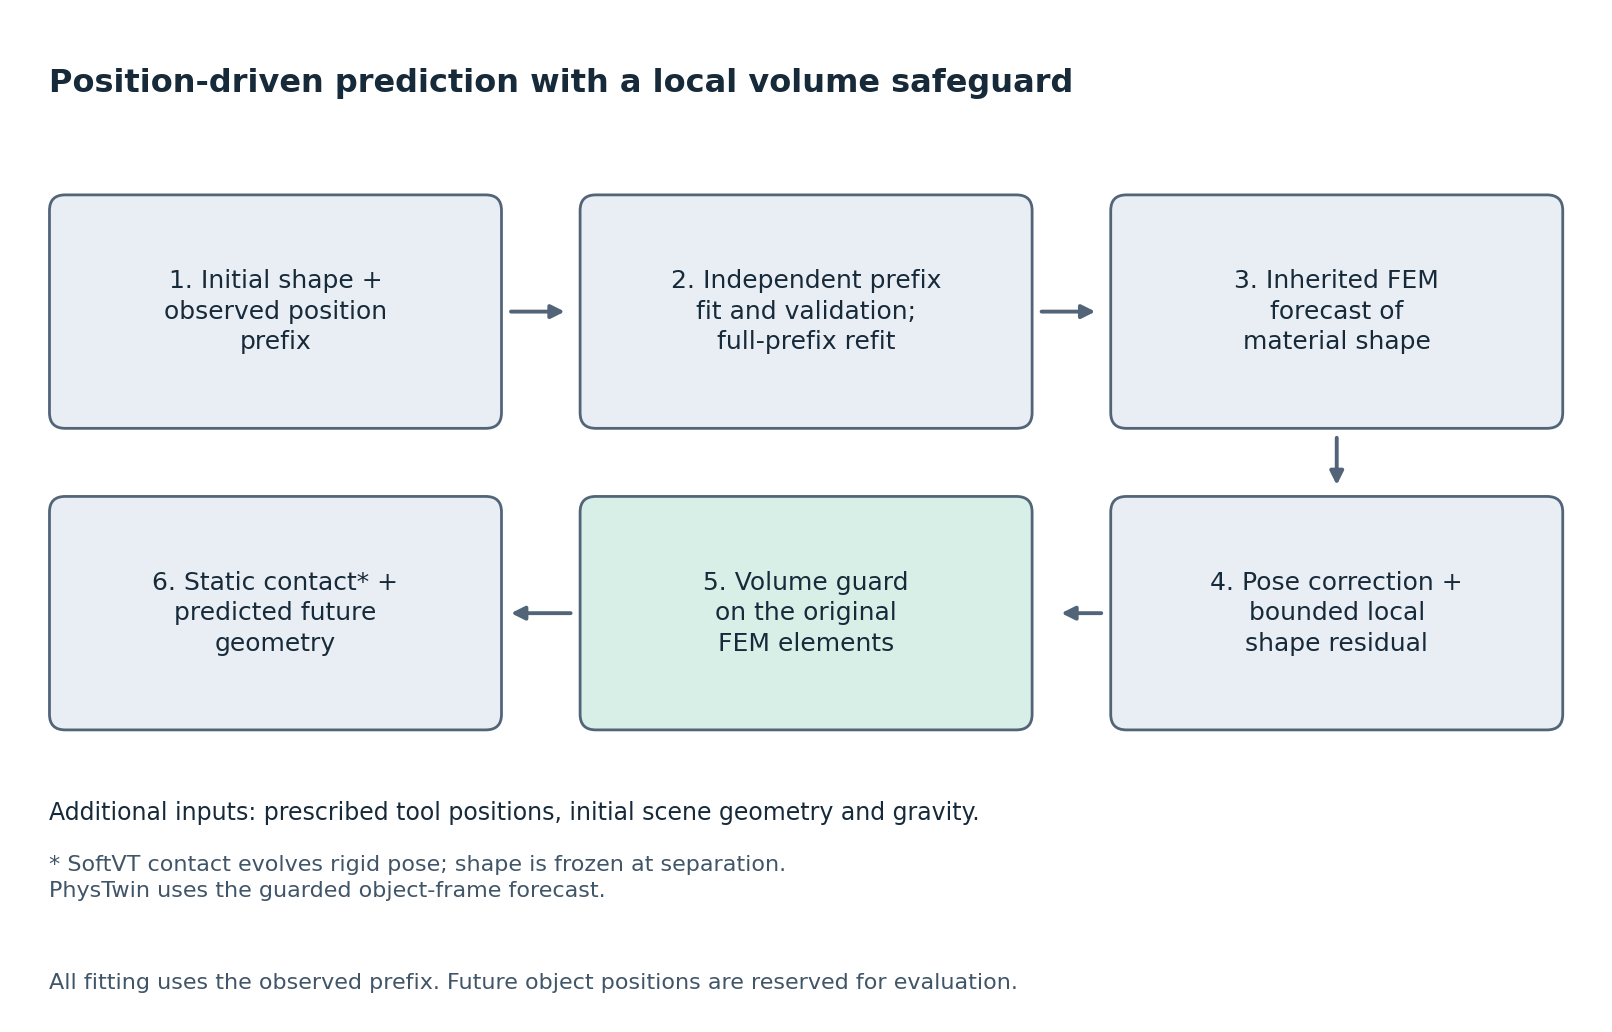
\includegraphics[width=\linewidth]{../../reports/contact-benchmark-v12/guarded-algorithm.png}
\caption{Implemented guarded prediction path. Observed-prefix calibration and prescribed tool positions produce a geometric forecast. The local volume guard is applied before reduced static contact; it does not turn that split model into a coupled elastic-contact solver.}
\end{figure}
A later mesh audit detected inverted inherited tetrahedra in some residual-corrected v12 trajectories. The preceding frozen method and its geometric scores remain archived; low geometric error does not make those trajectories mechanically feasible. A separate deterministic guard uses the original reference tetrahedra and signed volume ratios $J$. It backtracks the residual toward a rigidly aligned inherited FEM shape with a fixed coefficient schedule, requiring $J>0.03+10^{-8}$ before subsequent contact and velocity computation. This is a local saved-frame geometry safeguard, not an equilibrium solve or a continuous-time injectivity guarantee. Correction-induced velocity and acceleration changes are reported.

Re-evaluation of the original 106 sequences is explicitly post-audit secondary evidence. A separate 42-sequence cohort was declared before fetching its new PhysTwin data: SoftVTBench tasks 1--2, episodes 20--29 in both suites, and PhysTwin single-push sloth and double-lift zebra. These are new trajectories of known categories. The same frozen inference budgets and strong baselines are retained, including common scene postprocessing. No repaired-versus-original outcome is selected by future error.
\IfFileExists{generated-feasibility-results.tex}{\noindent Post-audit secondary extension: a deterministic original-tetrahedron volume guard is applied before contact. Frozen v12 remains unchanged. Only the additional 42 sequences are fresh confirmation; they share known object categories.
\par All required comparisons complete.
\begin{table}[ht]\centering\small
\resizebox{\linewidth}{!}{\begin{tabular}{llrrrr}\toprule
Dataset & Method & $n/N$ & Error(mm) & Shape(mm) & Failed frames \\\midrule
SoftVTBench & Frozen v11 FEM & 20/20 & 18.024 & 1.652 & 0 \\
SoftVTBench & Ours + scene contact & 20/20 & 15.199 & 1.417 & 0 \\
SoftVTBench & Feasible + scene contact & 20/20 & 15.372 & 2.096 & 0 \\
SoftVTBench & Rigid + scene contact & 20/20 & 15.402 & 0.924 & 0 \\
PhysTwin & Frozen v11 FEM & 1/1 & 39.401 & 19.175 & 0 \\
PhysTwin & Ours object frame & 1/1 & 34.076 & 17.333 & 0 \\
PhysTwin & Feasible object frame & 1/1 & 37.920 & 19.157 & 0 \\
PhysTwin & Official PhysTwin & 1/1 & 24.926 & 17.421 & 0 \\
\bottomrule\end{tabular}}
\caption{development. Full-suffix coordinate RMSE for SoftVTBench and manual-marker mean for PhysTwin; metrics not pooled.}
\end{table}
Guard changed 1562/2594 saved frames. Final inversion frames: 0; margin-violation frames: 0; nonfinite frames: 0. \par
\begin{table}[ht]\centering\small
\resizebox{\linewidth}{!}{\begin{tabular}{llrrrr}\toprule
Dataset & Method & $n/N$ & Error(mm) & Shape(mm) & Failed frames \\\midrule
SoftVTBench & Frozen v11 FEM & 40/40 & 26.967 & 1.922 & 0 \\
SoftVTBench & Ours + scene contact & 40/40 & 24.184 & 1.616 & 0 \\
SoftVTBench & Feasible + scene contact & 40/40 & 24.343 & 1.894 & 0 \\
SoftVTBench & Rigid + scene contact & 40/40 & 23.524 & 2.048 & 0 \\
SoftVTBench & Adapted PhysTwin + scene & 40/40 & 37.236 & 11.183 & 0 \\
PhysTwin & Frozen v11 FEM & 3/3 & 18.332 & 10.932 & 0 \\
PhysTwin & Ours object frame & 3/3 & 14.452 & 11.144 & 0 \\
PhysTwin & Feasible object frame & 3/3 & 16.146 & 10.885 & 0 \\
PhysTwin & Official PhysTwin & 3/3 & 13.155 & 10.368 & 0 \\
\bottomrule\end{tabular}}
\caption{regression. Full-suffix coordinate RMSE for SoftVTBench and manual-marker mean for PhysTwin; metrics not pooled.}
\end{table}
Guard changed 1293/5445 saved frames. Final inversion frames: 0; margin-violation frames: 0; nonfinite frames: 0. \par
\begin{table}[ht]\centering\small
\resizebox{\linewidth}{!}{\begin{tabular}{llrrrr}\toprule
Dataset & Method & $n/N$ & Error(mm) & Shape(mm) & Failed frames \\\midrule
SoftVTBench & Frozen v11 FEM & 40/40 & 23.531 & 1.943 & 0 \\
SoftVTBench & Ours + scene contact & 40/40 & 20.522 & 1.542 & 0 \\
SoftVTBench & Feasible + scene contact & 40/40 & 20.678 & 1.915 & 0 \\
SoftVTBench & Rigid + scene contact & 40/40 & 19.905 & 2.043 & 0 \\
SoftVTBench & Adapted PhysTwin + scene & 40/40 & 34.243 & 10.820 & 0 \\
PhysTwin & Frozen v11 FEM & 2/2 & 85.016 & 18.688 & 0 \\
PhysTwin & Ours object frame & 2/2 & 80.184 & 17.401 & 0 \\
PhysTwin & Feasible object frame & 2/2 & 81.985 & 18.665 & 0 \\
PhysTwin & Official PhysTwin & 2/2 & 26.218 & 16.304 & 0 \\
\bottomrule\end{tabular}}
\caption{untouched\_confirmation. Full-suffix coordinate RMSE for SoftVTBench and manual-marker mean for PhysTwin; metrics not pooled.}
\end{table}
Guard changed 752/5083 saved frames. Final inversion frames: 0; margin-violation frames: 0; nonfinite frames: 0. \par
\begin{table}[ht]\centering\small
\resizebox{\linewidth}{!}{\begin{tabular}{llrrrr}\toprule
Dataset & Method & $n/N$ & Error(mm) & Shape(mm) & Failed frames \\\midrule
SoftVTBench & Frozen v11 FEM & 40/40 & 23.971 & 1.939 & 0 \\
SoftVTBench & Ours + scene contact & 40/40 & 21.120 & 1.527 & 0 \\
SoftVTBench & Feasible + scene contact & 40/40 & 21.301 & 1.909 & 0 \\
SoftVTBench & Rigid + scene contact & 40/40 & 20.665 & 2.057 & 0 \\
SoftVTBench & Adapted PhysTwin + scene & 40/40 & 34.432 & 11.033 & 0 \\
PhysTwin & Frozen v11 FEM & 2/2 & 63.427 & 33.290 & 0 \\
PhysTwin & Ours object frame & 2/2 & 54.805 & 25.483 & 0 \\
PhysTwin & Feasible object frame & 2/2 & 60.395 & 33.173 & 0 \\
PhysTwin & Official PhysTwin & 2/2 & 26.164 & 14.594 & 0 \\
\bottomrule\end{tabular}}
\caption{fresh\_confirmation. Full-suffix coordinate RMSE for SoftVTBench and manual-marker mean for PhysTwin; metrics not pooled.}
\end{table}
Guard changed 825/5108 saved frames. Final inversion frames: 0; margin-violation frames: 0; nonfinite frames: 0. \par
}{\noindent Feasibility-extension result tables are pending; no numeric outcome is claimed.}

\FloatBarrier
\section{Exploratory selection of physical model complexity}
The numerical audit motivates a further, separately frozen experiment. A fitted global Gaussian potential can produce a large equilibrium-branch transition even with small equilibrium residuals and positive element volumes. Removing that term after fitting is not a valid remedy: parameters optimized with the term may be inappropriate without it. We therefore refit a second FEM family with only the Gaussian potential disabled. Gravity, material response, attachments, floor and the original compliant-support term remain present. A third, prefix-calibrated rigid family provides an explicit alternative when observed shape change is weak.

For each sequence, the first 70\% of the permitted observation prefix independently fits each FEM family. The remaining 30\% selects jointly among the physical family and the same fixed pose/residual adapter shortlist. Every candidate receives the local-volume guard and the same applicable static-contact processing before validation. The selector uses observed-position coordinate RMSE, without manual-marker targets, material labels or force measurements. A candidate must improve on the reconstructed prior configuration by strictly more than 2\%; ties retain the exact previously saved guarded prediction. Any invalid validation frame invalidates the whole candidate. If all candidates fail validation, the default remains and selection failure is recorded explicitly. A newly selected full-prefix model that fails remains a reported failure.

The selected configuration is then calibrated using the full permitted prefix and forecasts the unobserved suffix from prescribed positions. The rigid family has its own rigid anchor, so a failed deformable solve cannot invalidate it indirectly. Standalone family winners, selector choices, optimizer termination flags and per-case regressions accompany the selected-method scores. This experiment covers all 148 sequences and is entirely post-audit exploratory evidence: the earlier fresh-cohort designation does not transfer to this later model choice. It does not establish a permanent rigid/soft object classification or general coupled multi-object dynamics.
\IfFileExists{generated-model-selection-results.tex}{\begin{table}[ht]\centering\small
\resizebox{\linewidth}{!}{\begin{tabular}{llrrrrrrr}
\toprule
Cohort & Dataset & Complete/$N$ & Failed frames & v11 & Guarded & Selected & Rigid+scene & PhysTwin \\
\midrule
Development & SoftVTBench & 20/20 & 0 & 18.024 & 15.372 & 15.346 & 15.402 & NA \\
Development & PhysTwin & 1/1 & 0 & 39.401 & 37.920 & 37.116 & 75.252 & 24.926 \\
Regression & SoftVTBench & 40/40 & 0 & 26.967 & 24.343 & 23.984 & 23.524 & 37.236 \\
Regression & PhysTwin & 3/3 & 0 & 18.332 & 16.146 & 16.146 & 67.617 & 13.155 \\
Earlier cohort & SoftVTBench & 40/40 & 0 & 23.531 & 20.678 & 20.431 & 19.905 & 34.243 \\
Earlier cohort & PhysTwin & 2/2 & 0 & 85.016 & 81.985 & 35.514 & 57.373 & 26.218 \\
Later cohort & SoftVTBench & 40/40 & 0 & 23.971 & 21.301 & 21.069 & 20.665 & 34.432 \\
Later cohort & PhysTwin & 2/2 & 0 & 63.427 & 60.395 & 53.784 & 70.726 & 26.164 \\
\bottomrule\end{tabular}}
\caption{All rows are post-audit exploratory, including earlier confirmation cohorts. Means in millimeters; dataset metrics differ. Finite means with failed frames are conditional, not full-coverage performance. PhysTwin column is the common-scene adapted baseline on SoftVTBench and official reference on PhysTwin. Rigid uses scene contact on SoftVTBench; prefix nodal rigid on PhysTwin. NA denotes unavailable. Full-case/failure and complete-only means accompany the text report.}
\end{table}
}{\noindent Exploratory model-selection results are pending; no numeric outcome is claimed.}
\par\FloatBarrier
Across all 140 SoftVTBench sequences, mean forecast error decreases from 23.85\,mm for v11 to 21.15\,mm for the guarded extension and 20.90\,mm for model selection. The incremental gain is uneven: relative to the guarded extension, 41 sequences improve, 61 regress and 38 remain unchanged. The geometry-matched rigid baseline remains stronger at 20.51\,mm. On the 120 sequences with the adapted PhysTwin comparison, matched selector and adapted-baseline means are 21.83 and 35.30\,mm, respectively; this is a different cohort from the 140-sequence total.

On eight PhysTwin sequences, mean error decreases from 48.91\,mm for v11 to 46.39\,mm for the guarded extension and 33.02\,mm for model selection. Four sequences improve over the guarded extension and four remain unchanged. Approximately 87\% of the aggregate incremental gain comes from the previously diagnosed single-lift zebra case, which improves from 131.00 to 38.05\,mm. Official PhysTwin remains better on all eight cases, averaging 21.14\,mm. The simple position-ridge baseline also has a lower PhysTwin mean, 29.70\,mm. These results support a useful repair of model mismatch, while broader transfer remains unconfirmed.

All 148 selected forecasts are finite and retain positive tetrahedral volumes above the declared margin. Eight full-prefix and five shortened-prefix fits have abnormal optimizer termination flags; these remain disclosed rather than treated as converged optima. Standalone current-FEM forecasts are complete on 132/140 SoftVTBench and 7/8 PhysTwin cases; field-free forecasts are complete on 126/140 and 8/8, respectively. Their incomplete-cohort means are not full-coverage benchmark results. On the zebra case, an evaluator-only amendment records unavailable manual correspondence for the failed standalone current-FEM output without altering any saved prediction. Independent verification recomputes 592 forecast scores and checks all 296 new fits; a fixed 12-case replay reproduces selection metadata and forecast arrays exactly.
\IfFileExists{../../reports/contact-benchmark-v12/model-selection-comparison.png}{
\begin{figure}[ht]\centering
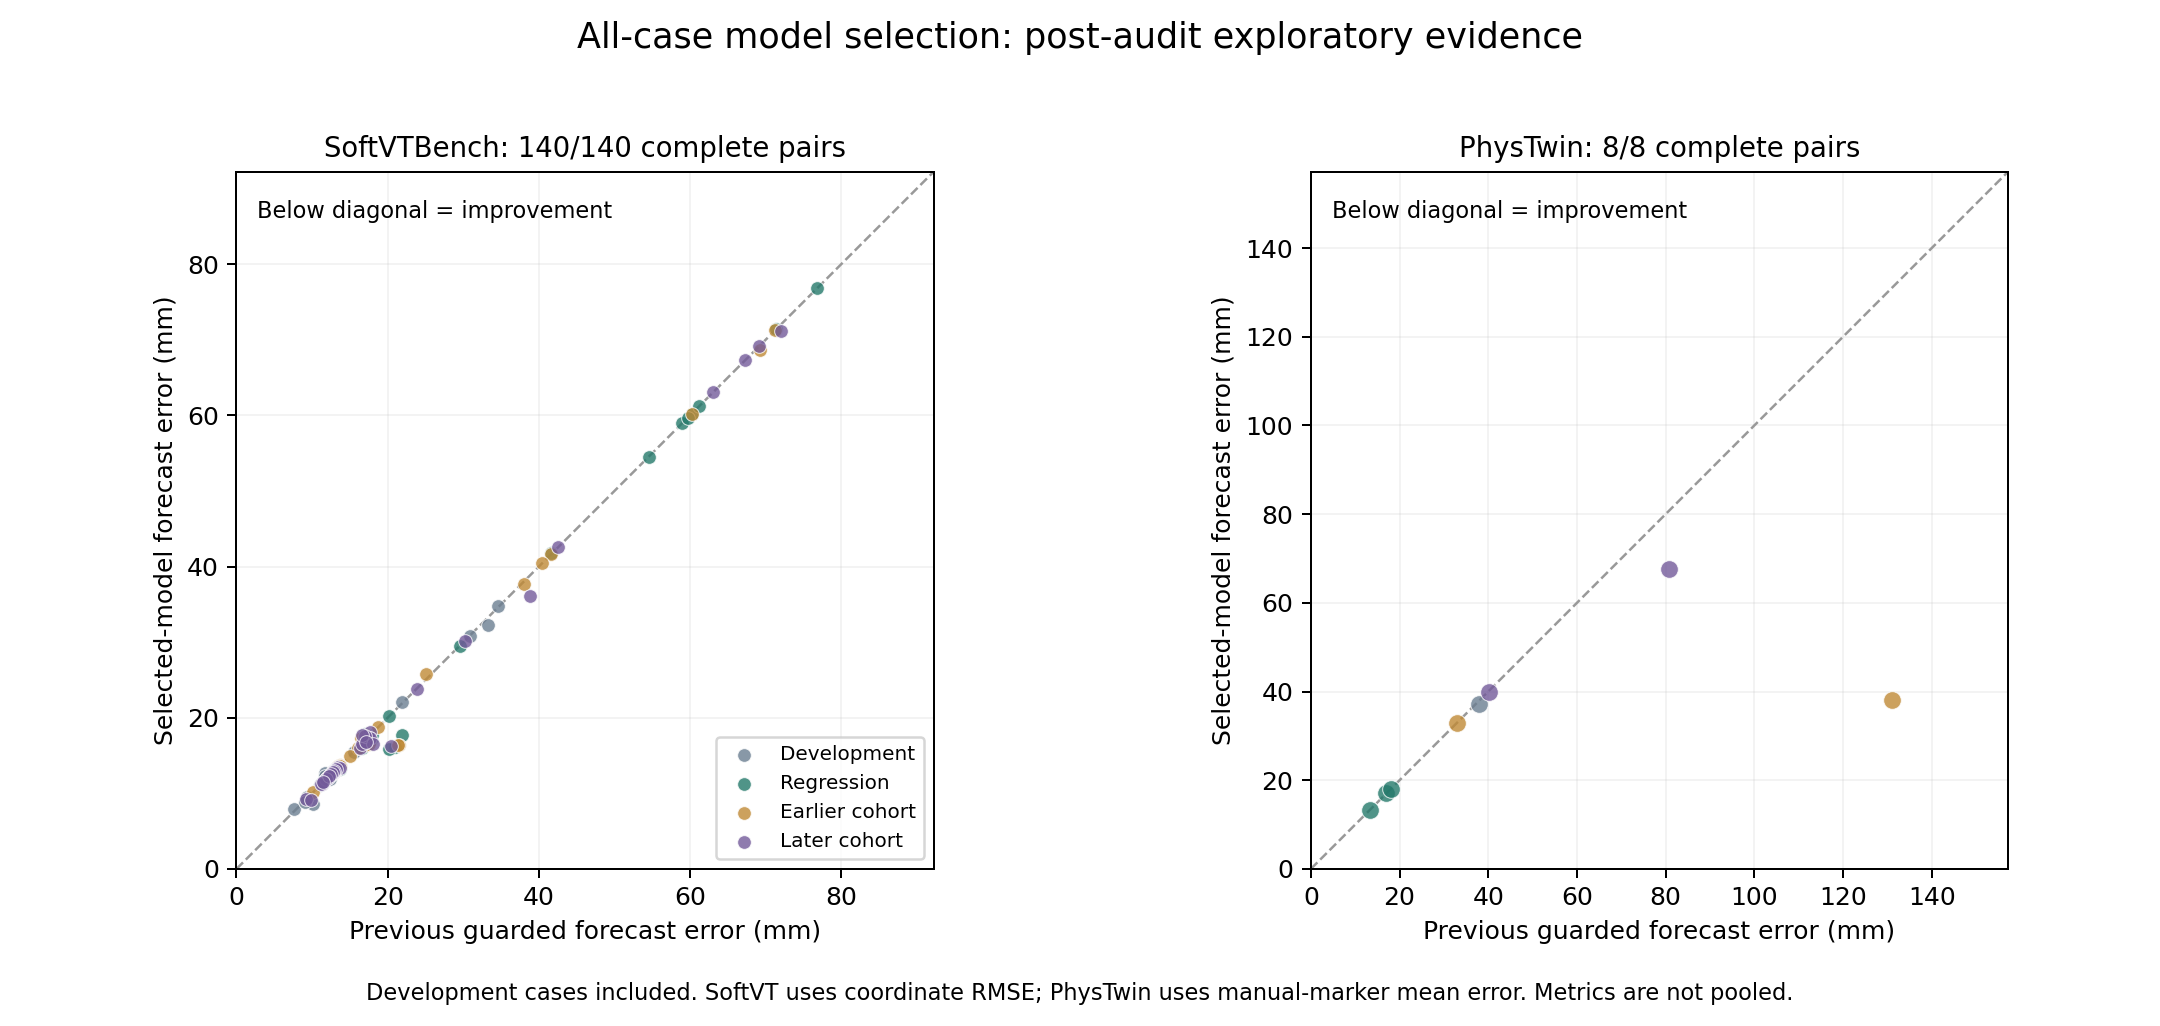
\includegraphics[width=\linewidth]{../../reports/contact-benchmark-v12/model-selection-comparison.png}
\caption{All complete sequence pairs for the exploratory selector. Each point compares the selected model with the previous guarded forecast. Dataset metrics are separate; any failed pairs are retained in the accompanying report.}
\end{figure}}{}

\FloatBarrier
\begin{thebibliography}{9}
\bibitem{phystwin} Hanxiao Jiang, Hao-Yu Hsu, Kaifeng Zhang, Hsin-Ni Yu, Shenlong Wang, and Yunzhu Li. \emph{PhysTwin: Physics-Informed Reconstruction and Simulation of Deformable Objects from Videos}. ICCV, 2025. \url{https://arxiv.org/abs/2503.17973}.
\bibitem{softvtbench} Bowen Jing et al. \emph{SoftVTBench: A Safety-Aware Visuo-Tactile Benchmark for Physically Constrained Robotic Manipulation of Deformable Objects}. arXiv:2607.04234, 2026. \url{https://arxiv.org/abs/2607.04234}.
\end{thebibliography}
\end{document}
